\chapter{Anhang}

\captionsetup{list=false}

\section*{Klassendiagramm}
\label{cha:anh:class}

\begin{figure}[H]
\centering
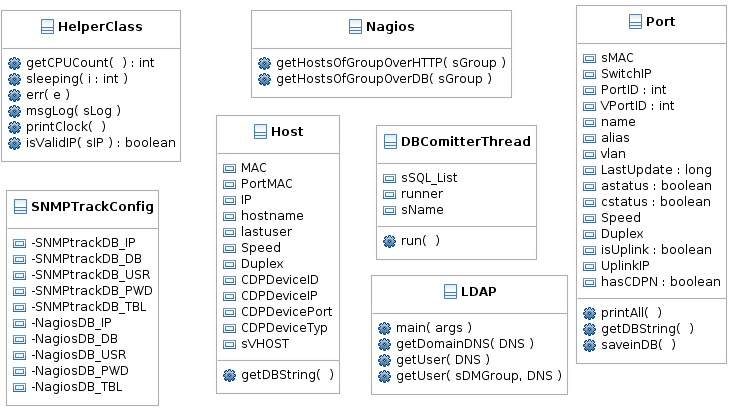
\includegraphics[width=1.0\textwidth]{model1.png}
\caption[]{Klassendiagramm}
\label{fig:classdia1}
\end{figure}

\begin{figure}[H]
\centering
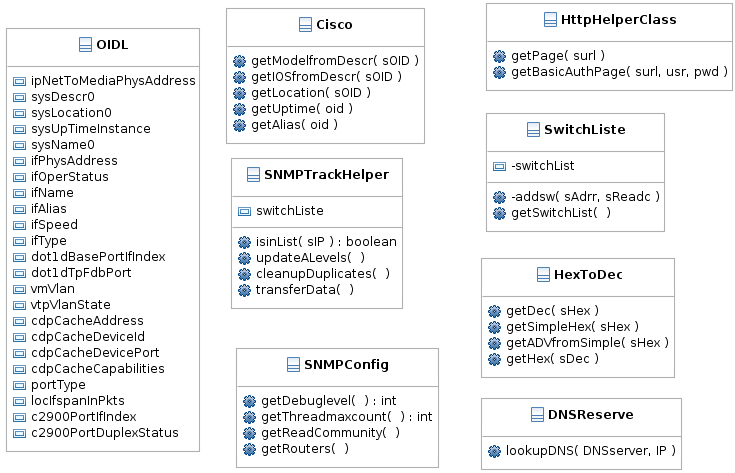
\includegraphics[width=1.0\textwidth]{model2.png}
\caption[]{Klassendiagramm}
\label{fig:classdia2}
\end{figure}

\begin{figure}[H]
\centering
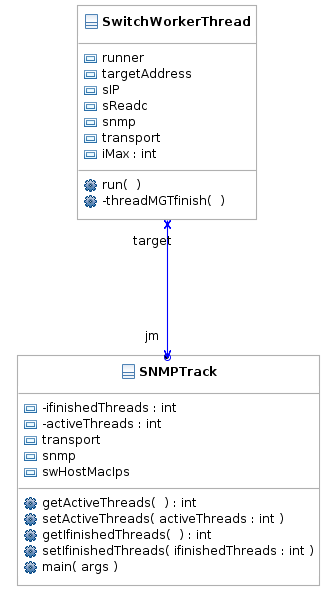
\includegraphics[width=0.4\textwidth]{model3.png}
\caption[]{Klassendiagramm}
\label{fig:classdia3}
\end{figure}

\begin{figure}[H]
\centering
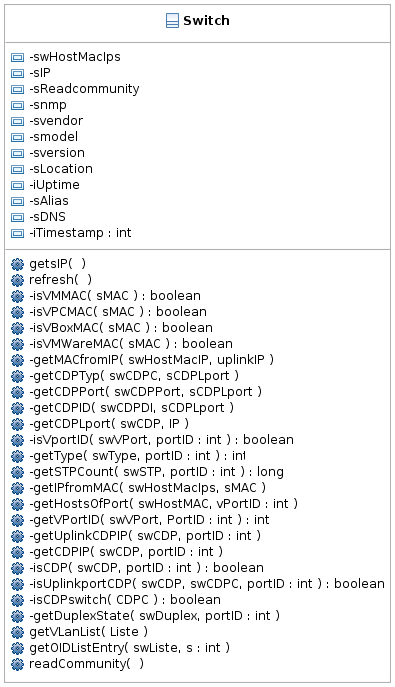
\includegraphics[width=0.6\textwidth]{model4.png}
\caption[]{Klassendiagramm}
\label{fig:classdia4}
\end{figure}

\begin{figure}[H]
\centering
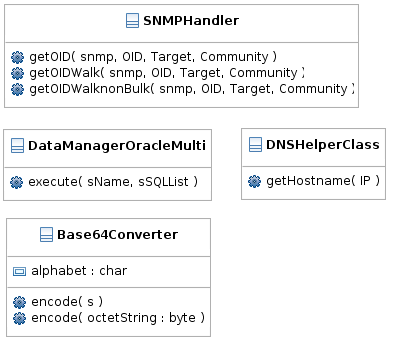
\includegraphics[width=0.6\textwidth]{model5.png}
\caption[]{Klassendiagramm}
\label{fig:classdia5}
\end{figure}

\begin{figure}[H]
\centering
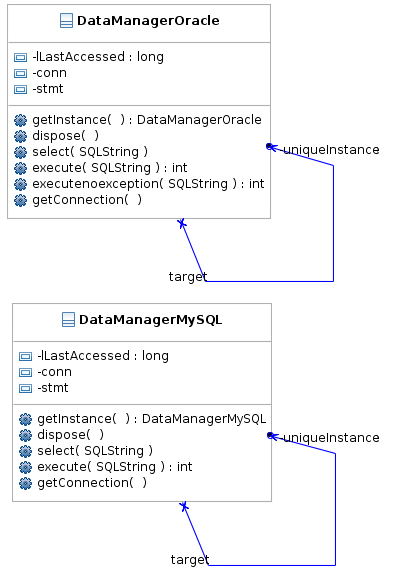
\includegraphics[width=1.0\textwidth]{model6.png}
\caption[]{Klassendiagramm}
\label{fig:classdia6}
\end{figure}

\section*{Konfiguration SNMP-Track}
\label{cha:Anhang1}

Noch leer.

\section*{Benchmarkwerte}
\label{cha:Anhang2}

Noch leer.